%!TEX root = slides.tex

\title{Emerging Technologies}
\subtitle{}
\author{ian.mcloughlin@gmit.ie}
\date{}


\begin{frame}
  \titlepage
\end{frame}

\begin{frame}
  \frametitle{Topics}
  \tableofcontents
\end{frame}

\section{Context}




\begin{frame}{Topology of software development}
  \begin{description}
    \item[Cloud infrastructure] Azure, AWS, Google Cloud, Heroku, Docker
    \vspace{0.25cm}
    \item[Web applications] Email, Social Networking, Enterprise software
    \vspace{0.25cm}
    \item[Mobile Application] Games, Fitness, Social, Productivity
  \end{description}
\end{frame}


\begin{frame}{Types of Programming Languages}
  \begin{description}
    \item[Scripting] Python
    \vspace{0.25cm}
    \item[Systems] Rust
  \end{description}
  \citeurl{spectrum.ieee.org/computing/software/the-2015-top-ten-programming-languages}
\end{frame}


\begin{frame}{Styles}
  \begin{center}
    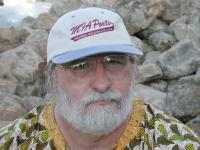
\includegraphics[width=1.4in]{img/richard-gabriel.jpg}
  \end{center}
  \begin{quote}
    I'm always delighted by the light touch and stillness of early programming languages.
    Not much text; a lot gets done.
    Old programs read like quiet conversations between a well-spoken research worker and a well studied mechanical colleague, not as a debate with a compiler.
    Who'd have guessed sophistication bought such noise? \\
    \hspace*\fill{\small--- Dick Gabriel}
  \end{quote}

  \citeurl{web.stanford.edu/class/ee380/Abstracts/100428-pike-stanford.pdf}
\end{frame}

\section{Go}
\begin{frame}[fragile]{Hello, World!}
  \begin{minted}{go}
package main
import "fmt"
func main() {
  fmt.Println("hello world")
}
  \end{minted}
  \citeurl{gobyexample.com/hello-world}
\end{frame}
